\section{View Maintenance Concept} 
\label{sec:view_maintenance} 


In this section, we develop techniques for maintaining the following
view types in our VMS: \texttt{SELECTION}, \texttt{PROJECTION},
\texttt{INDEX}, aggregation (i.e. \texttt{COUNT}, \texttt{SUM},
\texttt{MIN}, \texttt{MAX}, \texttt{AVG}) and join
(i.e. \texttt{INNER}, \texttt{LEFT}, \texttt{RIGHT},
\texttt{FULL}). Internally, VMS provides a number of auxiliary views,
which are the \texttt{DELTA}, \texttt{PRE-AGGREGATION} and
\texttt{REVERSE-JOIN} view, described
shortly. Figure~\ref{fig:view_types} gives an overview of all view
types and their dependencies.

Views at Level~1 directly derive from base tables residing at Level~0,
as indicated by the directed edges in the figure. A path along edges
from a base table to a view at a higher-numbered layer represents a
complete update path through the system.  More complex views on
Level~2 and higher are derived from views on lower layers, which, from
the perspective of these views, serve them as ``base data''.  Note
that there are alternatives in how certain view types can be
derived. For example, \texttt{SELECTION} can be derived from a base
table or from a \texttt{DELTA} view.  Dotted edges indicate that a
view type does not necessarily need to be materialized, as its
deriving table provides sufficient information to materialize the
given view on-the-fly without needing to scan table rows.  Determining
and quantifying the trade-offs among these view maintenance
alternatives is outside the scope of the present work.

In our below description, we use the extended relational algebra
notation to define views and update programs. View managers are
triggered by base table updates, which are submitted by clients. These updates are
denoted by $t_p$ and $t_d$ for put and delete, respectively, and $t_i$
and $t_u$ for insert and update, respectively.

\subsubsection{Auxiliary views}
\label{subsec:auxiliary_views}

Auxiliary views are internal to VMS and are not exposed to clients.
They are maintained to enable, facilitate and speed up the correct
maintenance of other view types.  Some views could not be maintained
consistently without the additional information provided by these
auxiliaries, others simply benefit from their pre-computations.  While
auxiliaries introduce storage overhead, they support modularity in 
view maintenance. Logically, auxiliaries represent the basic elements 
of view maintenance, which can be shared within and between view 
definitions. Thus, their use amortizes  as more
complexer views are managed by VMS.
%
% aj - above - modularity / locality is not clear
%
Auxiliaries also speed up view maintenance significantly, as we show
in Section~\ref{sec:evaluation}.

The update programs that compute the different view types make up most
of the view manger logic. In what follows, we describe each auxiliary
view type, including the problem it solves and how it is maintained
given base data updates.

\begin{figure}
  \centering
    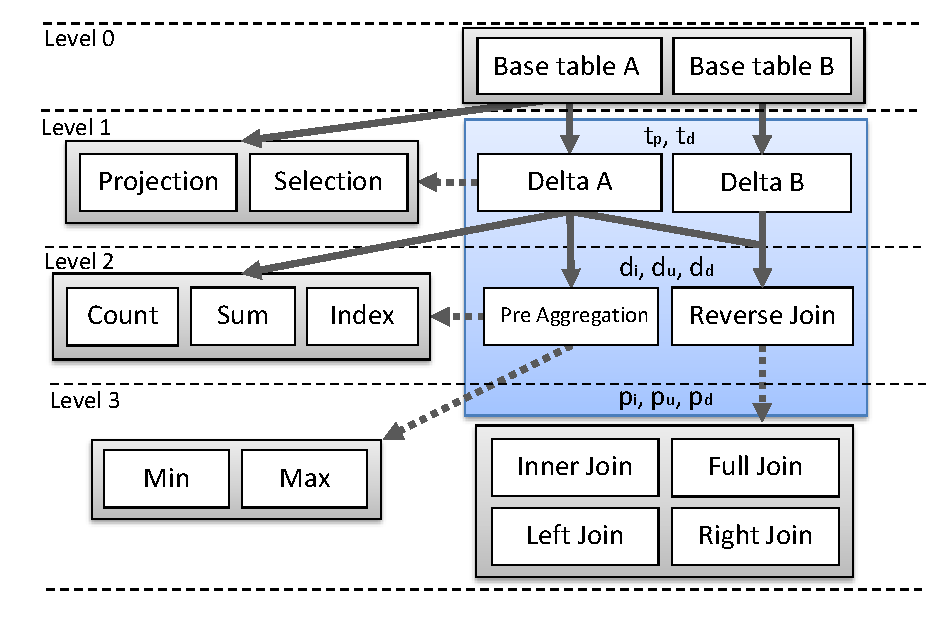
\includegraphics[width=\linewidth]{figures/ViewDependencies}
        \vspace{-5mm}
    \caption{View types and their dependencies}
        \vspace{-5mm}
    \label{fig:view_types}
\end{figure}


\noindent  
\textbf{Delta --} The \texttt{DELTA} view is an auxiliary view that
tracks base table changes between successive update operations.  Let
the base table be defined as $A = (\underline{K},F)$ and the view
table as $D=\delta_{c_1,c_2}(A)$.  The $\delta$ operator returns the
\textit{old} and the \textit{current} value for the specified columns;
here, old and current values for columns $c_1, c_2$. In 
Figure~\ref{fig:view_table_example} two examples of a \texttt{DELTA}
view are depicted.

%
% aj - above - more general notation, not restricting to c1/c2 would be better
%                     let it be for now.
% ja - i tried in the beginning, but it gets to messy, involves too many indices...

\noindent  
\textit{Motivation}: TL entries only contain the client operation.
They do not characterize the base record state before or after the
operation. For example, for a delete $t_d$, the client only provides
the row key, but not the associated value to be deleted, as input.
Likewise, an update operation provides the row key and new values, but
not the old values to be modified. In fact, a TL entry does not
distinguish between an insert and update operation, both are
represented by $t_p$. However, for view maintenance, this information
is vital. This motivated us to introduce the \texttt{DELTA} view. It
records base table entry changes, tracking the states between entry
updates, i.e., the ``delta'' between two successive operations for a
given row.  Views that derive, have this information available for
their maintenance operations.


\begin{figure*}
\minipage{1\textwidth}
  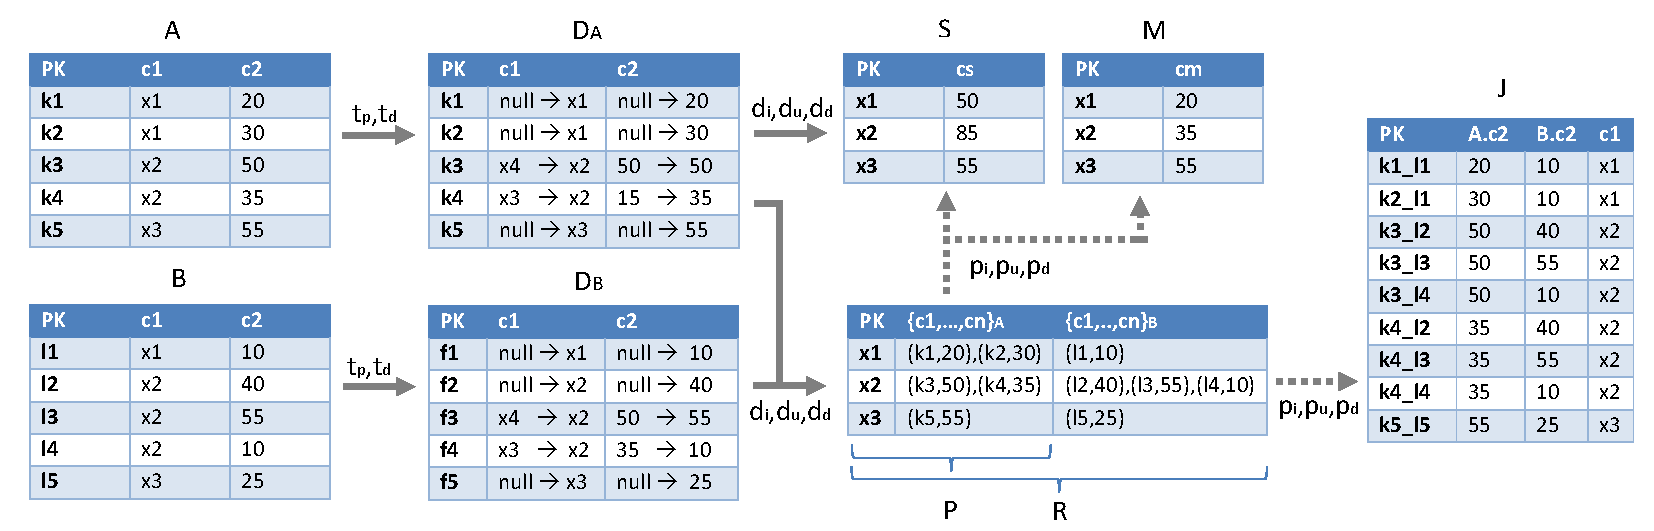
\includegraphics[width=\linewidth]{figures/ViewCalculationExample}
      \vspace{-7mm}
  \caption{View table example}\label{fig:view_table_example}
        \vspace{-5mm}
\endminipage\hfill
\end{figure*}

\noindent  
\textit{View update computation}: Now, we show the computation steps of 
the \texttt{DELTA} view when updated. As a general starting point, we 
create a base table and a view table (representing a particular view 
type) that is derived from the base table. We express view tables in the 
VMS with the help of relational algebra (e.g., we define a 
\texttt{SELECTION} as $\sigma_{c_1 < x}(A)$ over a base table $A$). As 
soon as the tables are set up, we insert a put operation $t_p$ and a 
delete operation $t_d$ into the base table. These two operation types 
are the only way a client can modify the base table and, hence, affect 
the view table. We denote the two operation types, as they are written 
to the TL, in the general form $t_p=put(A(k,\{\langle c_1, v_1\rangle, 
\langle c_2,v_2\rangle\}))$ and $t_d=delete( A(k))$. Once $t_p$ and 
$t_d$ are received by the VM, we discuss the VM's computation steps to 
update the view table. 

Client updates are either put or delete, $t_p$ or $t_d$ in our notation, 
respectively. The TL, entries $t_p$ and $t_d$ contain the following 
information, expressed in our as: $t_p=put(A(k,\{\langle c_1, 
v_1\rangle,\allowbreak \langle c_2,v_2\rangle\}))$ and $t_d=delete( 
A(k))$, respectively (i.e., base table name $A$, row key $k$, column 
name $c_i$, and value $v_i$.) 


Given the above defined view $D$, for both operations $t_p$ and $t_d$
on $A$, the VM performs a get on $D$ with row key $k$ to retrieve the
view record value state, i.e., $D(k\{ \langle c_1,v_1'\rangle, \langle
c_2,v_2'\rangle\})$. The value of the view record prior to the effect
of the current operation, i.e., the \textit{old} value, is annotated
with $'$, if it exists. If the record was newly inserted, no old value
exists and the return value is empty.  In this way, the VM can
distinguish between an insert, update or delete operation.  In case
$t_p$ is an insert (i.e., $t_i$), the query returns an empty result
for $c_i'$ and in case $t_p$ is an update (i.e. $t_u$), the query
returns the old value in $c_i'$.  Operation $t_d$ always is a
delete. It is identified by the current row value, $c_i$ of the transaction
being empty.

Now, depending on the type, $t_i$, $t_u$ or $t_d$, the VM performs the
following view updates, where ``$\Rightarrow$'' denotes the execution
of the VM based on the input and $\rightarrow$ represents the
transformation of a column's value from old to new:
%
\begin{eqnarray}
t_i & \Rightarrow  & put(D(k,\{\langle c_1,\emptyset \rightarrow v_1\rangle,\langle c_2,\emptyset \rightarrow v_2\rangle\}))\\
t_u & \Rightarrow & put(D(k,\{\langle c_1,v_1'\rightarrow v_1\rangle,\langle c_2,v_2' \rightarrow v_2\rangle\}))\\
t_d & \Rightarrow & put(D(k,\{\langle c_1,v_1' \rightarrow \emptyset\rangle,\langle c_2,v_2' \rightarrow \emptyset\rangle\}))
\end{eqnarray}
%
Operations applied to $D$ that may subsequently be consumed by views
derived from $D$, are denoted by $d$ (delta operation). They are
passed on as input to the KV-API by the VM, where again they are
written into the handling node's TL.  They do not only contain the 
client operation, but also the value that have been changed by that 
operation.
%
% aj - above - should we explain what additional info. they contain?
% ja - changed
In short, operation $t_i$ induces an operation $d_i$, $t_u$ induces
$d_u$ and $t_d$ induces $d_d$. In the following, we will make use of
this \texttt{DELTA} view output and the additional information it
provides.



\noindent  
\textbf{Pre-Aggregation --} The \texttt{PRE-AGGREGATION} view is an 
auxiliary view that prepares the aggregation by already sorting and 
grouping the base table rows. Consecutive aggregation views only need 
to apply their aggregation function, then.
%
% aj - above - ideally, we'd find a 1-liner to intuitively describe PA
% ja - tried my best
Let the \texttt{PRE-AGGREGATION} view $P$ be defined over the 
\texttt{DELTA} view $D$ as follows: $P=\gamma_{c_1,map\langle K,c_2\rangle}(D)$. 
A pre-aggregation can only be defined over a \texttt{DELTA} view, as it 
requires the values before and after client operations over base data. 
We use the relational algebra operator $\gamma_{x,f(y)}$ to express 
aggregates, where $x$ denotes the aggregation key and $f(y)$ denotes the 
aggregation function. When creating a pre-aggregation, we define a new 
aggregation function $map\langle K,c_2\rangle=\{\langle k_{x_1},v_{2x_1} 
\rangle..\langle k_{x_i}, v_{2x_i} \rangle\}_A$. The function takes a 
group of base records and stores into a map of key-value pairs. (A pair 
contains the row key and the aggregation value of the base record). This 
map is inserted into a single row in the view table by using a column 
family. In Figure~\ref{fig:view_table_example} an example of a 
\texttt{PRE-AGGREGATION} view is depicted. 



\noindent  
\textit{Motivation}: Often, an application calculates different
aggregations over the same aggregation key.  To materialize these
views, VMS must fetch the same record over and over. For \texttt{MIN}
and \texttt{MAX} views, the deletion of the minimum (maximum) in the
view requires an expensive base table scan to determine the new
minimum (maximum).  This motivated us to introduce the
\texttt{PRE-AGGREGATION} view. This view type sorts the base table
records according to the aggregation key, but stores the grouped rows
in a map.
%
% aj - above - notion of expaned is not clear
% ja - removed
Aggregation functions like \texttt{COUNT}, \texttt{SUM}, \texttt{MIN},
\texttt{MAX} or \texttt{AVG}, can then be applied to the map. They 
 will deliver the results instantaneously.
%
% aj - above - if again we have multiple rows, the aggregate them, 
%                    concurrent modifications may cause us grieve
% ja - no, we have test-and-set methods

\noindent  
\textit{View update computation}: The maintenance of a
pre-aggregation is triggered by the output of a delta view maintenance
step, fetched by a VM from a node's TL; that is, specifically by $d_i,
d_u$ and $d_d$.  Depending on this input, the VM performs the
following view updates:
%
\begin{eqnarray}
	d_i & \Rightarrow & put(P(v_1,\{\langle k,v_2\rangle, \langle k_{x_1},v_{2x_1}\rangle,..,\langle k_{x_i},v_{2x_i}\rangle\}))\\
	d_u & \Rightarrow & (v_1 = v_1')  \;\; \texttt{?} \;\; d_i \;\; \texttt{:} \;\; d_d \land d_i\\ 
	d_d & \Rightarrow & put(P(v_1',\{\langle k,\emptyset\rangle, \langle k_{x_1},v_{2x_1}\rangle,..,\langle k_{x_i},v_{2x_i}\}))
\end{eqnarray}
%
% Above From C's IF-Else shorthand: (integer == 5) ? (TRUE) : (FALSE);
% ja - changed 
When processing an update operation $d_u$, two cases must be
considered.  If the update does not change the aggregation key, then
simply a put is executed (i.e., $d_i$) on the KV-API. However, if the aggregation
key is changed, then a delete with the old key is executed, followed
by an insert (i.e., $d_d \land d_i$).
%
% aj - above - need to think about the case (not sure I follow)
% ja - if the aggregation key changes we need to delete the delta from the
%	   old key and apply it to the new one (two operations). If only the value
%	   is changed, we can just update the aggregatio key (one operation)

Operations applied to $P$ that may be consumed by views derived from
$P$, are denoted by $p$ (pre-aggregate operation). They are passed on
as input to the KV-API by the VM, where again they are written into
the handling node's TL.  They contain the complete map of grouped values
to be processed by following views. When base records are aggregated 
moderately, computation runs fast. But if there are many row keys and 
only a few aggregation keys, update operations tend to grow very large. 
In this case, we might as well store the \texttt{PRE AGGREGATION} view
together with all the aggregation views (\texttt{COUNT},\texttt{SUM}, etc.).
Then, the aggregation view is nothing but another column in the table
of the \texttt{PRE AGGREGATION} view. Considering 
Figure~\ref{fig:view_types}, this saves a complete level of computation.

%
% aj - above - is it correct? It is a variant of what was said above
%                  - should we explain what additional info. they contain?
%                  - do we need the below? It would need to be adapted.               
% In short, operation $t_i$ induces an operation $d_i$, $t_u$ induces
% $d_u$ and $t_d$ induces $d_d$. In the following, we will make use of
% this \texttt{DELTA} view output and the additional information it
% provides.




\noindent  
\textbf{Reverse Join (2-tables) --} A \texttt{REVERSE-JOIN} view is an
auxiliary view that supports the efficient and correct materialization
of join views in VMS.  A \texttt{REVERSE-JOIN} view supports the
maintenance of a join between two tables: $A \bowtie B_{A.c_1=B.c_1}$,
with Join key in column $c_1$ of tables $A$ and $B$.  Let the base
tables and their respective delta views be defined as follows:
$A=(\underline {K},F_A)$, $B=(\underline{L}, F_B)$,
$D_A=\delta_{c_1,c_2}(A)$, and $D_B=\delta_{c_1,c_2} (B)$. Then, the
\texttt{REVERSE-JOIN} view is defined as $R=\gamma_{c_1, map\langle K,c_2
  \rangle, map\langle L,c_2\rangle}(D_A,D_B)$. Figure~\ref{fig:view_table_example}
 shows an example of a \texttt{REVERSE JOIN} view. 

\noindent  
\textit{Motivation}: A \texttt{JOIN} view is derived from at least two
base tables. For an update to one of these tables, the VM needs to
query the other base table to determine the matching join rows. Only
if the join-attribute is the row key of the queried base table, can
the matching row be determined quickly, unless of course, an index is
defined on the join-attribute for the table.  Otherwise, a scan of the
entire table is required, which has the following drawbacks: (i) Scans
require a disproportional amount of time, slowing down view
maintenance. (With increasing table size, the problem worsens.) (ii)
Scans keep the nodes occupied, slowing down client requests.  (iii)
While a scan is in progress, underlying base tables may change, thus,
destroying view data consistency for derived views. To address these 
issues, we introduce the \texttt{REVERSE-JOIN} view.

We take the \textit{join key} ($jk$) of the two base tables as row key
of the \texttt{REVERSE-JOIN} view. When updates are propagated, the
\texttt{REVERSE-JOIN} view can be accessed from either side of the
relation with the help of the join key (it is always included in both
tables' updates). If a record is inserted into one of the underlying
base tables, it is stored into the view --- whether or not it has a
matching row in the other base table.

In this way, \texttt{INNER}, \texttt{LEFT}, \texttt{RIGHT}, and
\texttt{FULL} can derive from the \texttt{REVERSE-JOIN} view without
the need for base table scans, as we show below.

\noindent  
\textit{View update computation}: Client operations $t_i$, $t_u$ and
$t_d$ are either issued to $A$ or to $B$. In both cases, operations
are inserted into the TL and updates are applied to the \texttt{DELTA}
view $D_A$ or $D_B$. Let $D_A$ produce the operations $d_i, d_u, d_d$.
Then, the view manager updates the \texttt{REVERSE-JOIN} view as
follows:
%
\begin{eqnarray}
	d_i & \Rightarrow & put(R(v_1,\{\langle k,v_2\rangle\}_A, \{\langle l_{y_1},v_{2y_1}\rangle,..,\langle l_{y_j},v_{2y_j}\rangle\}_B))\\
	d_u & \Rightarrow & \;\; (v_1 = v_1') \;\; \texttt{?} \;\; d_i \;\; \texttt{:} \;\; d_i \land d_d\\ 
	d_d & \Rightarrow & put(R(v_1',\{\langle k,\emptyset\rangle\}_A, \{\langle l_{y_1},v_{2y_1}\rangle,..,\langle l_{y_j},v_{2y_j}\rangle\}_B))
\end{eqnarray}
% 
Operations that are produced from $D_B$ are treated analogously.
We are using column families $\{..\}A$ and $\{..\}B$ in the join view
to separate updates from different base tables. Later, this
facilitates the computation of the matching join rows, for we only
need to combine the records of the two families. After the operations
are applied to the \texttt{REVERSE-JOIN} view, they are also
pre-aggregated (by the join key) and we denote them with $p$. As 
Figure~\ref{fig:view_table_example} indicates, \texttt{PRE-AGGREGATION} 
view is contained in the \texttt{REVERSE-JOIN} view. In fact, both 
views are conceptually the same. This opens up
potential for savings in storage and computation. If both views are
derived from the same table and if the aggregation key is the same
as the join key, we can simply put them together. 



\noindent  
\textbf{Reverse Join (n-tables) --} We discussed the \texttt{REVERSE 
  JOIN} view, which joins two base tables by a join key.

For joining $n$ tables, we have to distinguish two cases: (i) Join all
tables on the same join key and (ii) base tables are joined on
different join keys.  In the former case, we just need to extend the
2-table definition to $n$ tables. Let the \texttt{REVERSE-JOIN} view
be defined as $R_n=\gamma_{c_1,
  map\langle K,c_2\rangle, map\langle L,c_2 \rangle,..map\langle X,c_2\rangle}(D_A,D_B,..,
D_{\Phi})$. For every new join table $\Phi$ with \texttt{DELTA} view
$D_{\Phi}$, a new column family is added to the view. This column
family collects the updates of the base table.  As long as we are
joining on the same key, we can put all relations to the same
\texttt{REVERSE-JOIN} view.

In the latter case, base tables are joined on different join keys. For
example, $A \bowtie B \bowtie C$, where table $A$ and $B$ are joined
on column $c_1$, whereas table $B$ and $C$ are joined on a column
$c_3$.  To enable this, we have to combine multiple
\texttt{REVERSE-JOIN} views. We are free to choose, whether we build a
\texttt{REVERSE-JOIN} for $A \bowtie B$ and combine the result with
$C$ or we build a \texttt{REVERSE-JOIN} for $B \bowtie C$ and combine
it with $A$. For every pair of distinct join keys, we need a
\texttt{REVERSE-JOIN} view.  In the worst case, we have $n$ join
tables and $n-1$ distinct join keys, resulting in the same number of
\texttt{REVERSE-JOIN} views.  However, this compositional manner of
deriving join views, leads to a number of possible optimizations. When
computing join $A \bowtie B \bowtie C$ and $B \bowtie C \bowtie D$,
relation $B \bowtie C$ only needs to be computed once, for instance.



\subsubsection{Standard views}
\label{subsec:common_views}

In this section, we describe how VMS maintains client-exposed views
for a number of interesting standard view types. We also present
alternative maintenance strategies, but defer a full-fledged cost
analysis to future work.

\noindent  
\textbf{Selection and Projection --} A \texttt{SELECTION} view selects
a set of records from a base table based on a \textit{selection
  condition}.  The row key of the base table serves as the row key of
the view table and a single base record uniquely maps to a single view
table record.  Let a selection view be defined as $S=\sigma_{c_2 <
  v_x}(A)$, where the selection condition is $(c_2 < v_x)$ requiring
that selected values in column $c_2$ are smaller than $v_x$.  The view
manager processes operations $t_p$ and $t_d$ as follows:
%
\begin{eqnarray}
	t_p & \Rightarrow & t_d\;\land\;\;(v_2 < v_x)\;\; \texttt{?} \;\;put(S(k_1,\langle c_1,v_1\rangle, \langle c_2,v_2\rangle))\\
	t_d & \Rightarrow & delete(S(k))
\end{eqnarray}
%
% aj - above - let us verify the notation, why use t_d and also delete(S(K))
% ja - I just want to point to the delete (no redundancy). Below are cases,
%	   where the t_d is very long and i don't want to repeat the whole op
A record delete is performed for every operation on the view.  This is
because, the selection condition cannot be evaluated on the operation,
as it may not contain the value.  For $t_d$, the VM does not know the
deleted value and cannot determine, if there is a corresponding view
record. For $t_p$, the VM is not able to distinguish between an insert
vs. an update.  Thus, in both cases, the VM pre-emptively deletes the
record in the view.

A \texttt{PROJECTION} view selects a set of columns from a base
table. Similar to the \texttt{SELECTION} view, the VM uses the row key
of the base table as row key for the view table.  Let a view table be
defined as $P=\pi_{c_2}(A)$, then, the VM determines the update for
$P$ given $t_p$ and $t_d$ as follows:
%
\begin{eqnarray}
	t_p & \Rightarrow & t_d\;\land\;\;put(P(k_1, \{\langle c_2,v_2\rangle)\})\\
	t_d & \Rightarrow & delete(P(k))
\end{eqnarray}
%
Pre-emptive deletes are executed for the same reasons as above.

An alternative maintenance strategy is to derive both views from a
\texttt{DELTA} view. We create a \texttt{DELTA} view
$D=\delta_{c_1,c_2}(A)$ and define the \texttt{SELECTION} view as
$S=\sigma_{c_2 < v_x}(D)$ and likewise the \texttt{PROJECTION} view as
$P=\pi_{c_2}(D)$. This alleviates the need for pre-emptive deletes,
since the VM always receives the complete row state. The computation
of the \texttt{SELECTION} view changes to:
%
\begin{eqnarray}
	d_i \land d_u & \Rightarrow & \;(v_2 < v_x)\;\; \texttt{?} \;\;put(S(k_1,\langle c_1,v_1\rangle, \langle c_2,v_2\rangle))\\
	d_d                & \Rightarrow & (v_2 < v_x)\;\; \texttt{?} \;\;delete(S(k))
\end{eqnarray}
%
The computation of the \texttt{PROJECTION} view changes analogously
when derived from a \texttt{DELTA} view. To save storage and
computation resources, we could combine \texttt{DELTA},
\texttt{PROJECTION} and \texttt{SELECTION} into one view. This would
reduce the amount of records (due to selection), the amount of columns
(due to projection), and still provide delta information to subsequent
views. These considerations are important for multi-view optimization
in VMS, which we defer to future work.


\noindent  
\textbf{Count and Sum --} The maintenance of \texttt{COUNT} and
\texttt{SUM} views is very similar, so we treat them together.
Generally speaking, in aggregation views, records identified by an
\textit{aggregation key} aggregate into a single view table record.
The aggregation key becomes the row key of the view. Let a base table
$A$ and $D$ be defined as before. Then, a \texttt{SUM} view is defined
as $S=\gamma_{c_1,Sum(c_2)}(D)$. Note, the view is defined over a
delta table and not a base table. The row key of table $S$ is the
aggregation key of the view (i.e. the value of $c_1$).  Operations
$d_i,\;d_u$ and $d_d$ are processed as follows: The view manager
queries $S$ to retrieve the last state of the aggregated value, e.g.,
$S(v_1',\{\langle c_s,v_s'\rangle\})$. Then, the VM computes the new
state of the aggregated value by adding the ``delta'', i.e.,
$v_s=v_s'+(v_2 - v_2')$. In case the update operation changed the
aggregation key (i.e., $v_1' \neq v_1$), the update involves two
records in the view table. Thus, the VM executes a delete on the old
key $v_1'$ and an insert on the new key $v_1$. A \texttt{COUNT} view
is a special case of a \texttt{SUM} view. Updates for it results by
setting $v_2=1$ and $v_2'=1$ in the following updates for
\texttt{COUNT}:
%
\begin{eqnarray}
	d_i &\Rightarrow& put(S(v_1,\{\langle c_s,v_s'+ v_2\rangle\}))\\
	d_u &\Rightarrow& (v_1 = v_1')\;\; \texttt{?} \;\;put(S_1(v_1',\{\langle c_s,v_s'+ (v_2 + v_2')\rangle\}))\\
	 &&\texttt{:} \;\;\delta(t_i) \land \delta(t_d)\notag\\ 	
	d_d &\Rightarrow& put(S(v_1',\{\langle c_s,v_s'- v_2'\rangle\}))
\end{eqnarray}
% 
\textit{Example 1:} Given tables $A$, $D$ and $S$ as before (i.e., view 
tables are defined as $D=\delta_{c_1, c_2}(A)$ and 
$S=\gamma_{c_1,Sum(c_2)}(D)$). Let the initial table states be given as 
depicted in Figure~\ref{fig:view_table_example}. Let the client perform 
an update operation on row key $k_2$, which is inserted into $A$ 
resulting in the entry $t_1 \in T$ in the TL. Let 
$t_1=put(A(k_2,\allowbreak\{\langle c_1,x_2\rangle,\langle c_2,15 
\rangle\}))$. At this point, it is not know whether $t_1$ is an insert 
or an update operation (both operations could result from a put.) Once 
$t_1$ is processed on the delta view $D$ by a view manager, another 
entry $t_2 \in T$ is created in the TL. Being induced by $t_1$, $t_2$ 
captures the changes to row $k_2$ as $t_2=put(S(k_2,\{\langle c_1,x_1 
\rightarrow x_2\rangle,\langle c_2,30\rightarrow 15\rangle\}))$. Note, 
$t_2$ now identifies the client operation as an update. Operation $t_2$ 
triggers an update on $S$. Because the operation changes the aggregation 
key, the VM generates an update statement for aggregation key $x_1$ and 
$x_2$. To execute the first statement, the VM queries the view table and 
retrieves $S(x_1,\{\langle c_s,50) \rangle\})$. It computes $50 - 30 = 
20$ and puts $S(x_1, \{\langle c_s,20\rangle\})$ to update view table 
$S$. To execute the second statement, the VM queries the view table and 
retrieves $S(x_2,\{\langle c_s,85)\rangle\})$. It computes $85 + 50 = 
135$ and puts $S(x_2, \{\langle c_s,135\rangle\})$ to update view table 
$S$.  


Alternatively, a \texttt{SUM} and \texttt{COUNT} view could be derived
from a \texttt{PRE-AGGREGATION} view.  Let
$P=\gamma_{c_1,map\langle K, c_2\rangle}(D)$ and define the \texttt{SUM} view $S$
as $S=\gamma_{c_1,SUM(map\langle K, c_2\rangle)}(P)$. Now, the \texttt{SUM} view is
maintained for a given $p$ as follows:
%
\begin{eqnarray}
	p_{i/u} & \Rightarrow& put(S(v_1,\{\langle c_s, (v_2 + v_{2x_1}+..+v_{2x_i})\rangle\}))\\
	p_d & \Rightarrow& put(S(v_1,\{\langle c_s, (v_{2x_1}+..+v_{2x_i})\rangle\}))
\end{eqnarray}

%
% aj - below - the term secondary key is not correct, it would refer to 
%                    a base table column that could be used instead of the
%                    primary key, i.e., its values are unique; our index view
%                    is more general, it can index any base table column.
%
\noindent
\textbf{Index --} \texttt{INDEX} views are important to provide fast
access to arbitrary columns of base tables. The view table uses the
chosen column as row key of the view, storing the corresponding table
row keys in the record value. If the client wishes to retrieve a base
table row by the indexed column, it accesses the \texttt{INDEX} view
first, then, it accesses the base table with the row keys retrieved
from the record found in the view. This is a fast type of access, for
the client is always accessing single rows by row key. The
\texttt{INDEX} view is a special case of the \texttt{PRE-AGGREGATION}
view. If the indexed key is the same as the aggregation key, we can
combine both view types. Further, the \texttt{PRE-AGGREGATION} can be
combined with a \texttt{REVERSE-JOIN} view (see description above).
Thus, we receive three different view types at the cost of one.


 
\noindent  
\textbf{Min and Max Views --} \texttt{MIN} and \texttt{MAX} views are
also aggregates. Both can be derived from a \texttt{DELTA} or a
\texttt{PRE-AGGREGATION} view. When derived from a \texttt{DELTA}
view, \texttt{MIN} and \texttt{MAX} are computed similar to a
\texttt{SUM}. However, a special case is the deletion of a minimum
(maximum) in a \texttt{MIN} (\texttt{MAX}). In that case, the new
minimum (maximum) has to be determined. Without the assistance of
auxiliary views, a table scan would have to be
performed~\cite{jacobsen:viewmaintenance}. This motivated us to derive
the \texttt{MIN} (\texttt{MAX}) from a \texttt{PRE-AGGREGATION}, which
prevents the need for a scan.  Let tables $A$, $D$ and $P$ be defined
as before.  Then, a \texttt{MIN} view is defined as
$M=\sigma_{Min(c_2)} (P)$. The \texttt{MIN} is updated as follows:
%
\begin{eqnarray}
	p_{i/u} & \Rightarrow& put(S(v_1,\{\langle c_s, min(v_2, v_{2x_1},..,v_{2x_i})\rangle\}))\\
	p_d & \Rightarrow& put(S(v_1,\{\langle c_s, min(v_{2x_1},..,v_{2x_i})\rangle\}))
\end{eqnarray}

\noindent
\textbf{Join --} The \texttt{JOIN} view presents the results of $n$ 
joined base tables. Since the matching of join partners has been already 
completed in the \texttt{REVERSE JOIN} view, the \texttt{JOIN} view is 
used to display results in a proper way. To get the join result, the VM 
takes the output operations of the \texttt{REVERSE JOIN} view and 
multiplies their column families. Thereby, the \texttt{INNER}, 
\texttt{LEFT}, \texttt{RIGHT}, \texttt{FULL} join can be constructed. 
Let the \texttt{JOIN} view be defined over the \texttt{REVERSE JOIN} 
view as $J=\gamma^{-1}_{(K,L), map\langle K,c_2\rangle \times 
map\langle L,c_2\rangle}(R)$. In Figure~\ref{fig:view_table_example} an example 
of a \texttt{JOIN} view is depicted. We use notation $\gamma^{-1}$ to 
indicate that the VM is doing the exact opposite of an aggregation at 
this point. It takes two (or multiple) column families of a single row 
and creates a set of result rows by building the cross product. While 
building the cross product, the view manager combines the row keys of 
both base tables to form a composite key ($(K,L)$). Likewise, it includes the 
$c_2$ values of both base tables in the result. The update operations 
are executed by the view manager as follows: 
%
\begin{eqnarray}
		p_i,p_u& \Rightarrow& put(J(k_{x_1}l_{y_1},\{\langle c_1, v_{2x_1} \rangle,\langle c_2, v_{2y_j} \rangle\})),\\
		 	&&...\notag\\
		 	&&put(J(k_{x_i}l_{y_j},\{\langle c_1, v_{2x_i} \rangle,\langle c_2, v_{2y_j} \rangle\}))\\	
		p_d& \Rightarrow& delete(J(k_{x_1}l_{y_1})),...,delete(J(k_{x_i}l_{y_1}))	 	 	
\end{eqnarray}
%
\noindent 
In order to build the different join types, the view manager varies
the update computation as follows:
{\renewcommand\labelitemi{}
\begin{itemize}
\setlength{\itemindent}{-.05in}
\item \textbf{Inner}: Cross product $\{..\}A$ and
  $\{..\}B$, neither $\{..\}A=\emptyset$ nor $\{..\}B=\emptyset$
\item \textbf{Left}: Include rows with $\{..\}B=\emptyset$
\item \textbf{Right}: Include rows with $\{..\}A=\emptyset$
\item \textbf{Full}: Include rows with either
  $\{..\}A=\emptyset$ or $\{..\}B=\emptyset$
\end{itemize}
}


%
% aj - above - seems incomplete
%                   - discussion of join views is not really understandable

%\noindent
%\begin{itemize}[label={}]
% \setlength{\itemindent}{-.2in}
% \setlength{\itemsep}{0em}
%	\item \textit{Inner join:}
%	\begin{subequations}
%  		\begin{align}
%		  r_i \Rightarrow& put(J(k_1l_{y_1},\{\langle c_1,v_2(k_1) \rangle, \langle c_2,v_2(l_{y_1})\rangle%\})),\notag\\&...,put(J(k_1l_{y_j}, \{\langle c_1,v_2(k_1) \rangle, \langle c_2,v_2(l_{y_j})\rangle\}))\notag\%\
%		  r_u \Rightarrow& r_i \land r_d\notag\\
%		  r_d \Rightarrow& delete(J(k_1l_{y_1})),..delete(J(k_1l_{y_j}))\notag	
%		\end{align}
%	\end{subequations}
%	
%	\item \textit{Left join:} Include updates, with $\{..\}B=\emptyset$ 
%	\item \textit{Right join:} Include updates, with $\{..\}A=\emptyset$ 
%	\item \textit{Full join:} Include updates, with $\{..\}A=\emptyset$ and $\{..\}B=\emptyset$ 
%\end{itemize}


%
%\noindent  
%\textbf{Nested Views --} As shown in Figure~\ref{fig:viewdependencies}, 
%our basic set of views already relies on nesting. For example, 
%aggregation views depend on a \texttt{DELTA} view, which itself depends 
%on the base table. Starting with the base tables, located at Level~0, we 
%can build more complex view hierarchies. Given view tables simply serve 
%as input for other derived views. An update at Level~0 (base table) 
%triggers updates to Level~1 views and so on. For example, we can compose 
%a \texttt{JOIN} and a \texttt{SUM} view. The flow of updates is 
%consistent, because the per-key order is preserved and the updates of 
%dependent views occurs along the specified view hierarchy. Moreover, we 
%can profit from the modular design and reuse view computations multiple 
%times. The \texttt{PRE AGGREGATION} view can be used to model all types 
%of aggregation views, including an \texttt{INDEX} view. The calculations 
%of a \texttt{JOIN} view $A \bowtie (B \bowtie C)$ can also be part of 
%the $(B \bowtie C) \bowtie D$. The \texttt{REVERSE JOIN} view $(B 
%\bowtie C)$ defines the relation between $B$ and $C$ and can produce the 
%output for various subsequent materialized views. 


